\chapter{Breathing}

\keywords{brief \emph{ānāpānasati} method and posture}

\noindent We watch the sensations of the breathing in the body, this
alert attention collects the mind around a stable object. The physical
sensations in the body are easy to notice as we breathe in- and out.
This is the method of mindfulness of breathing (\emph{ānāpānasati}).

Why is thinking so exhausting? The mind is jumping from thought to
thought, but we don't know where we're going, and so, we never arrive.
Restless desire is exhausting. Sense-restraint gathers energy and
directs it instead of letting it flow out in every direction. Directing
attention to a neutral, steady sensation like the breath slows down the
thinking mind.

One may sit on the floor, using a mat and a cushion, or on a chair.
Sitting on the floor, find a position which doesn't over-stress the
tendons or the knees.

When using a chair, move forward on the seat so that your back is not
leaning against the back-rest. A support influences the shape of the
spine and the rhythm of the breathing.

\enlargethispage*{\baselineskip}

Balance the head so that its weight is not pulling forward. Since we
often sit on chairs, we have a habit of holding the head in a forward
position, which creates tension in the back muscles. When we pull the
head backward, we can feel the back muscles relaxing. Pull in the chin
slightly, but there is no need to force it.

\clearpage

\begin{figure}[h]
\caption{Mindfulness of Breathing (\emph{Ānāpānasati})}\label{fig-mindfulness-of-breathing}
\bigskip\centering
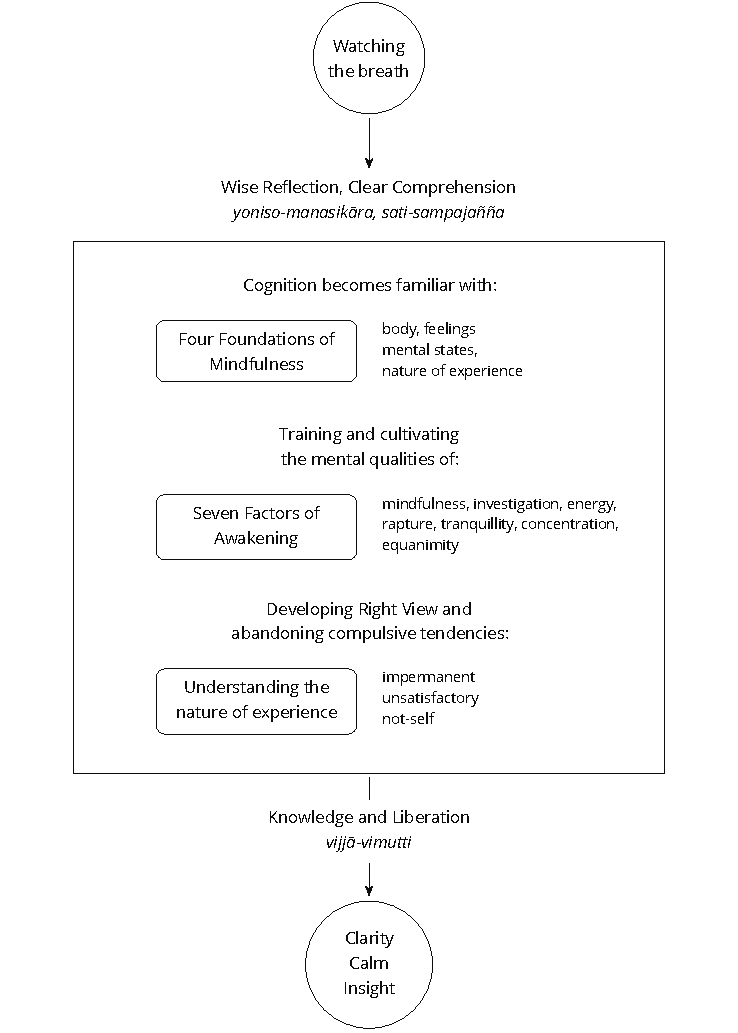
\includegraphics[scale=0.7]{mindfulness-of-breathing.pdf}
\end{figure}

\clearpage

Sit in a balanced, upright posture, with the shoulders relaxed. In a
good posture, the breathing is easy and even.

The bones in the body sit on top of one another like a tower of stones.
The hip-bone rests on the cushion, the spine on the hip, the spine disks
stacked on one another, with the skull on top, the centre-line of the
whole tower carefully held in balance.

When balanced carefully with its weight at the centre, we don't have to
hold up the body by pulling or pushing with the strength of muscles.
Gravity is enough to keep it upright.

Breathing in, the cold air touches the tip of the nose. Let the
abdominal muscles draw in the breath instead of expanding the chest to
gain volume. The air moves through the lungs, and the abdomen expands.
This way of breathing lowers the heart rate and reduces anxiety.
Relaxing the muscles, air leaves through the nostrils. There is no need
to control it with precision, it is enough to suggest this rhythm. The
body already knows how to breathe, so we take a step back and observe,
like watching waves wash in onto the shore, and then recede.

We don't have to tell ourselves what to think and how to feel. If we
want clear thoughts, it is best to first be silent and listen. We sit
and rest for a little while. When we are silent, either clear thoughts
will come on their own, or the mind will be content to stay with the
silence.

Restraint and directed attention is necessary for clear, conscious
thought -- and it brings a peaceful gladness with it. The mind is
content and happy, we don't need much internal discussion. Sitting and
breathing, listening to the silence is a blameless joy in itself.

We establish a clear intention to stay with the meditation object and
leave other matters until a later time. An open attitude is helpful,
pushing and forcing ourselves is not sensitive enough to see what is
happening. Operating from will-power makes the meditation rigid, and the
mind obstructed. Like marching fast with stiff legs, and falling over on
small pebbles.

A clear mind and good aspiration feels settled and cool, the attitude is
open to change. Forcing and struggling feels busy, hot and narrow in
scope.

\keywords{attitude toward the method, mind is not a coffee machine}

Are we learning new facts about the mind by observing the breathing? I
remember when I sat down and struggled to understand how to meditate
\emph{correctly}. I kept thinking about this, changing my breathing to
improve my meditation, expecting that one day I will somehow hit the
correct buttons, and breathing in the correct way I will start learning
new information, new facts about the mind. It was rather painful and
entirely fruitless.

Analysing it for knowledge we miss what is happening. Think about a
conversation, when the other person keeps asking ``Why?'' after your
every sentence -- the conversation goes nowhere without listening.
Overthinking it, we are doing this to ourselves, and no wonder we want
to jump up from the cushion and tell our commentating mind to stop and
listen in silence.

The instructions from our teachers are a guide for directing attention
in a way to discover understanding for ourselves.

We learn from the instructions we read or hear, but trying to follow
them \emph{exactly, precisely, correctly} is more like following a
manual to operate a coffee machine: `if I press this button, it should
always make this kind of coffee'.

This attitude is motivated by the desire to control and manipulate our
experience, but we experience the frustration because by nature we don't
have control over it. We already decided what will happen. We want to
see what we \emph{think} should happen, and we don't see what \emph{is}
happening, so we think the machine is not working, or we are doing it
wrong.

We can remind ourselves that it is possible that we don't know
everything. We don't know what is going to happen. Loosen the hold,
practice an attitude of stopping and listening.

\keywords{BUD-DHO mantra, effort and frustration}

We may start with practising the BUD-DHO mantra, internally repeating it
with the in- and the out-breath. `Buddho' means `one who is awake, one
who is knows'. It helps to stop and listen.

This wakes up the mind to know the mind as it is right now, and waking
up is always right -- you can't do it wrong. The mind recognizes its own
changing nature, the words of thinking are no longer necessary, and
attention finds the wordless question which stays with the present.

Effort is necessary, and the obstructions in the mind can make it hard
work to not quit the practice. Again and again, we return to the mind
which is awake to the present experience to guide effort, rather than
wilful pushing towards a goal.

Frustration and disappointment are useful indicators to listen -- the
best is when we have to learn something we didn't expect to learn.

We don't have to read or remember much. The information we need is
little, but developing skill in them requires much practice. We don't
stop to stay with them, and unpack their significance for recognizing
our situation, \emph{what} to do, and \emph{in what way} to do it.

A list of facts, if not integrated, doesn't reach deep enough to deal
with root causes in the heart and mind, and have no effect on us.
Watching the breath stops us and opens the attention which can do that.
Perception and recognition can be gradual, like having to lean close to
something to see an essential feature, but every step, which connects
our experience with the words of the teachings, is interesting and leads
onward.

The Buddha has a simple message for us: wake up, stop holding on, you
don't have to suffer. We keep unpacking this, unfolding it wider and
wider.

\section{Guided meditation}

\keywords{\emph{ānāpānasati} method, sitting meditation, sitting posture}

Adjust how you sit and find a balanced posture: an upright position, in
a stable but not tense posture, with the head balanced and not lulling
forward. The posture should allow open, easy breathing.

Determine that you are putting down everyday activities for this period.
You can respond to interrupting thoughts, `This is not the right time, I
will come back to that when the time is appropriate.' It's a bit longer
than `Go away!', but more friendly to ourselves. This establishes a
clear intention in the mind, like when clearing a desk before starting
work.

Take a deep breath and watch if you feel tension, something obstructing
or limiting the breath. If you feel that the breathing is easy and open,
then your posture is suitable. You don't have to sit in a special way.

Pay attention to the physical sensation of breathing. Let the body
regulate the breath. We watch and let it relax, giving attention to what
is happening now.

Good posture and the calm, easy breathing is a quiet and pleasant
feeling, like sitting down on a park bench after a walk. There nothing
special to do, and this simple, quiet sitting is a joy in itself.

We don't control the breathing so precisely as in a pranayama or yoga
exercise, but it is worth noticing the bodily rhythm which drives our
breathing.

If the breathing is driven by the expansion and contraction of the
chest, as if we were preparing for a great effort, this creates energy
to move and produces a more actively thinking mind. It has a calming
effect when the diaphragm above the abdomen controls the breathing. Once
you find the rhythm of it, let the body continue.

Breathing in, we first feel the air at the nostril. The cold air moves
down in the windpipe. The abdomen moves outward, allowing the diaphragm
to expand. The chest rises as the air fills the lungs, but we're not
expanding the chest to a great volume. Sitting still, we can feel the
quiet rhythm of heartbeats.

Breathing out, the muscles relax, the warm air rises through the wind
pipe, and leaves through the nose.

It is not necessary to express these steps in thought, relax and watch
as the feelings appear in the body. It can take a little while for the
body to settle. The beating of the heart will calm down, and the
breathing becomes regular and light.

Allow the body to regulate the breathing on its own. When we approach it
with an opinion, that our breathing should be short or long, then it
becomes rigid and forceful. We want to discover our experiences, not
tell them what they should be.

The body knows how to breathe better than we do. It will breathe with an
even rhythm, if we let it. Take a step back and turn the attention
around, listening instead of directing. Breathing in, breathing out,
what are you feeling in the body?

It is not one specific feeling which you have to experience. The
intention is to give the time and allow the space to be with your
experience.

Centred within itself, knowing the simplicity of the present moment. The
feeling that we have to complete, or fix something, is always an extra,
something which we create. We create this expectation that we have to
change, we have to fix, we have to control. This is always connected to
time, we expect something which should happen.

In the present moment everything is moving, going through change. In the
immediate, present experience there are no goals. There are not results
to come in the future, there is only \emph{this, here}. The expectations
which we produce for ourselves, dissolve, when we return our attention
and watch the present.

We return to the attention connected to the experience here and now. It
recognizes the world through the senses. In this attention the doubts,
questions, memories, are not heavy. They don't have such weight, such
urgent importance, which would move us out from the centred balance.
This wakeful attention becomes a secure place where we can stay.

There may be a lot of tangled thinking in the mind. Determine what to
think, instead of letting the mind run in circles. For example, use the
mantra BUD-DHO. On the in-breath, think BUD-, on the out-breath, -DHO.
If the thinking doesn't slow down on its own, this puts down a guard
rail and speed bumps, so that we stay on track and slow down.

\keywords{active and calm mind, turbulent emotions, simplicity of the present}

Breathing in, staying with the simple experience of the moment, this is
enough.

We feel compulsions, desires and anxieties, we feel `I need this', `I am
like this', `I should be like that'. They are something we can observe,
we don't need to get involved in the story. Staying with the breathing,
we can turn attention to the experience that is happening.

Awareness of the body is a solid base, calming and reorganizing what is
valuable. If your experience is peaceful, happy and content, stay with
that. There is nothing wrong with that. This happiness is not connected
to craving, not dependent on having to get or reach something. It arises
from seclusion of the senses, returning to simplicity, knowing and
staying with the present. The mind is alert, content, and satisfied.

Meditation can bring up turbulent emotions, and that is good. We are
seeing what we haven't allowed ourselves to see. Looking for answers or
solutions is not necessary while meditating. We don't investigate the
emotions on the level of our personal history, but on a more fundamental
level, as states of the mind and heart.

We see ourselves in them, we see them as ours, and we create a person,
whose story we want to control. But in the present moment neither the
feeling, nor the mind state makes any announcement about whose name they
belong to. The suffering and difficulty comes from this attachment and
confused perspective. We have to open the mind to the change, and let go
of the attachment.

\keywords{wholesome thoughts, being too serious}

Virtue, generosity relaxes the mind, and morality establishes stability.
We may think of good actions, what we have given and received. We may
recollect people we look up to as good examples with respect.

If you find yourself in a tense, strict and cynical mood, try shifting
your posture to relax.

We can get so serious about sitting on a cushion, it is a living joke to
look at us. Quietly rub your ears or massage the face muscles using your
fingers, this invigorates blood flow. Recollect generosity. In the
monastery, often our lay friends are coming to cook and offer the midday
meal for the community. They can be busy while in the kitchen, but when
finished, they are at ease, relaxed and smiling.

The mind can be anxious for results, and recollecting our good actions,
even simple and small ones, relaxes that tension. Imagine what would
happen, if someone gave you a hundred-times-fold of the results you
want, such as winning an enlightenment lottery. How are you going to
meditate then? Probably much like now, but more relaxed. Grant yourself
that rich, wide space.

Generosity lets us recognize that we already have space, and don't have
to push to get ahead of others. Goodness is present in the world and we
can drop the big hurry. It feels joyful to recollect the generosity of
our family, relatives and friends, but even seeing a stranger help
another stranger brings us to smile.

\keywords{doubt in meditation, senses turning inward}

`How can I do it?' Approach it differently, and ask instead, `Can I pay
attention to it?'

The sensation of breathing stops us. We are back at the beginning, when
we didn't know what is going to happen. We are at an empty and spacious
place this way, where we are by ourselves and we have time to stop
there.

The senses turn inward when watching the breathing. The eye sees
colours, but the attention of seeing turns inward, and not seeking
colours and forms outside. The ear hears sounds, but the hearing turns
inward and is not seeking. The body feels hot and cold, the surface of
clothes and the rigid weight of the bones. We watch this while breathing
and let the body calm down, let the mind turn inward and grow still.

\keywords{cool water filling a lake, experience contains the world}

Sense-restraint collects our energy and doesn't let it flow away in
every direction. Consider a lake which doesn't have inlets or outlets,
contained all around by the valley. Its single water-source is a fresh,
cool spring in the ground. When it rains, some water will flow into the
lake through small channels, but there being no outflow, it will all
settle in the lake contained by the valley. The water in the lake
remains still, and the cool water from the spring will spread and
permeate the entire lake.\footnote{\href{https://suttacentral.net/dn2}{DN
  2}, The Fruits of the Ascetic Life}

Feelings and the mind are dependent on the body, we can't add to it or
take away from it. Experience is complete in every breath, it starts
with the body and is going to end with it. This world, made of feelings,
is complete in this -- it contains everything we are and everything we
can ever become.

\keywords{awareness stops compulsion}

When we suffer, we know that there is something we don't understand. We
don't understand how one thing is created by another, how one thing is
under our control, and another is not.

When we don't see, we repeat the pattern like following a program, and
create the same suffering again and again. We complain, `why does it
always happen this way?' We keep doing the same thing, and not see it.

Looking closer, we see that one thing depends on another. Then we can
see the option, that we are free to stop doing it. We return to a quiet
contentment this way.

\keywords{restlessness, self-criticism, beginning with good will, flexible attitude}

When we have been sitting in meditation for a while, we often start to
complicate it. Where does this restlessness come from, can we not stay
with something simple? Notice how belief in the simple experience
changes. We start thinking about some point or question, and the doubt
and self-criticizing stops everything.

Isn't it comical? We can be so committed to our self-criticism, as
though it was a transcendental experience to cause ourselves pain. But
we feel we should be struggling with \emph{something}, we should crush
our ego and let go of everything! Perhaps this is the only way we know,
we never thought we could be different.

At the beginning we have good will and flexible attitude to ourselves,
but there is only hardness and judgement at the end. The young tree is
pliant and fresh, it bends as it grows, but the old tree is hard and dry
when it dies.

Return to the beginning, when you had kindness and patience toward the
beginner. You didn't yet expect yourself to know what to do, and relied
on listening to see what happens. We don't know what is here until we
look and see. That seeing and watching is the fresh knowing. Allow
yourself to always be at the beginning.
